\documentclass{article}

\usepackage{amsfonts}
\usepackage{graphicx}
\usepackage{amssymb}
\usepackage{amsmath}

\setlength\parindent{18pt}

\begin{document}


Textbook Section 2.1:

22) Suppose that at time $t = 0$, half of a "logistic"
population of 100,000 persons have hard a certain rumor, and that the
number of those who have heard it is then increasing
at a rate of 1000 persons per day. How long will
it take for this rumor to spread to 80\% of the population?
(Suggestion: Find the value of $k$ by substituting
$P(0)$ and $P'(0)$ in the logistic equation, Eq. (3).)


Equation 3:

\[\frac{dP}{dt} = kP(M-P)\]

where $k = b$ and $M = \frac{a}{b}$ are constants.


$M = 100,000$, $P(0) = 50,000$, $P'(0) = 1,000$.

\[1,000 = k \cdot 50,000(100,000 - 50,000)
\implies 1 = k \cdot 50(50,000)\]
\[\implies k = \frac{1}{2,500,000}\]


\[\frac{dP}{dt} = kP(M-P)\]
\[\int \frac{dP}{P(100,000-P)} = \int k \cdot dt\]
\[-\frac{ln(|\frac{100,000}{P}-1|)}{100,000} + C = kt\]
\[ln(|\frac{100,000}{P}-1|) + C = -100,000kt\]
\[ln(|\frac{100,000}{P}-1|) = -100,000kt + C\]
\[e^{ln(|\frac{100,000}{P}-1|)} = e^{-100,000kt + C}\]
\[|\frac{100,000}{P}-1| = e^{-100,000kt + C}\]
\[|\frac{100,000}{P}-1| = A \cdot e^{-100,000kt}\]
\[\frac{100,000}{P} = 1 \pm (A \cdot e^{-100,000kt})\]
\[P = \frac{100,000}{1 \pm (A \cdot e^{-100,000kt})}\]

\[P(0) = 50,000\]
\[\implies P = \frac{100,000}{1 + (1 \cdot e^{-100,000kt})}\]
\[\implies P = \frac{100,000}{1 + e^{-100,000kt}}\]


\[P(t) = \frac{100,000}{1 + e^{-100,000kt}}\]


$80\%$ of population = $0.8 \cdot 100,000 = 80,000$
Solve for $t$:
\[P(t) = 80,000\]
\[\frac{100,000}{1 + e^{-100,000kt}} = 80,000\]
\[\frac{1}{1 + e^{-100,000kt}} = \frac{4}{5}\]
\[\frac{5}{4} = 1 + e^{-100,000kt}\]
\[\frac{5}{4} - 1 = e^{-100,000kt}\]
\[\frac{1}{4} = e^{-100,000kt}\]
\[ln(\frac{1}{4}) = -100,000kt\]
\[-\frac{ln(\frac{1}{4})}{100,000} = kt\]
\[t = -\frac{ln(\frac{1}{4})}{100,000k}\]

\[t \approx 34.657\]


$80\%$ of people will have heard a certain rumor after approximately $34.657$ days.



Textbook Section 2.2:

5) $\frac{dx}{dt} = x^2 - 4$

\[\frac{dx}{dt} = 0\]
\[\implies x^2 - 4 = 0\]
\[\implies (x+2)(x-2) = 0\]
\[x = \pm 2\]

\[x'(-3) = 5\]
\[x'(0) = -4\]
\[x'(3) = 5\]


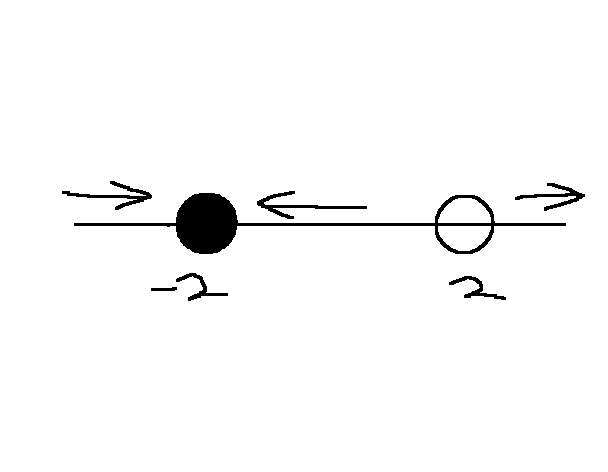
\includegraphics[width=\linewidth]{problem_5}



\[\int \frac{dx}{x^2 - 4} = \int dt\]
\[\frac{ln(|x-2|) - ln(|x+2|)}{4} + C = t\]
\[ln(|x-2|) - ln(|x+2|) + C = 4t\]
\[ln(|\frac{x-2}{x+2}|) = 4t + C\]
\[|\frac{x-2}{x+2}| = e^{4t + C}\]
\[\frac{x-2}{x+2} = A \cdot e^{4t}\]
\[x-2 = (A \cdot e^{4t})(x+2)\]
\[(-A \cdot e^{4t})x + x - 2 = 2A \cdot e^{4t}\]
\[(-A \cdot e^{4t})x + x = 2A \cdot e^{4t} + 2\]
\[(1-A \cdot e^{4t})x = 2A \cdot e^{4t} + 2\]
\[x = \frac{2A \cdot e^{4t} + 2}{1-A \cdot e^{4t}}\]



7) $\frac{dx}{dt} = (x-2)^2$

\[\frac{dx}{dt} = 0\]
\[\implies (x-2)^2 = 0\]
\[x = 2\]


\[x'(1) = 1\]
\[x'(3) = 1\]


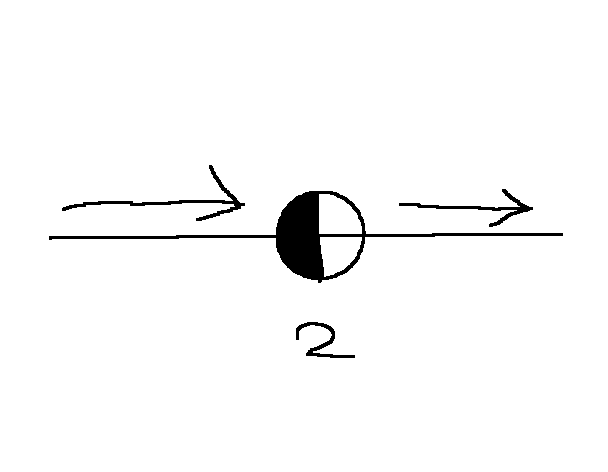
\includegraphics[width=\linewidth]{problem_7}



\[\int \frac{dx}{(x-2)^2} = \int dt\]
\[-\frac{1}{x-2} + C = t\]
\[-t + C = \frac{1}{x-2}\]
\[x-2 = -\frac{1}{t + C}\]
\[x = 2 - \frac{1}{t + C}\]



9) $\frac{dx}{dt} = x^2 - 5x + 4$

\[\frac{dx}{dt} = 0\]
\[\implies x^2 - 5x + 4 = 0\]
\[\implies (x-4)(x-1) = 0\]
\[x = 1, x = 4\]

\[x(0) = 4\]
\[x(2) = -2\]
\[x(5) = 4\]


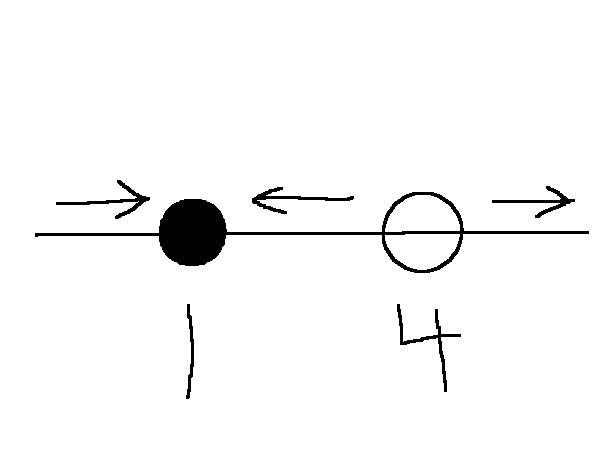
\includegraphics[width=\linewidth]{problem_9}



\[\int \frac{dx}{(x-4)(x-1)} = \int dt\]
\[\frac{ln(|\frac{3}{x-1} - 1|)}{3} + C = t\]
\[ln(|\frac{3}{x-1} - 1|) + C = 3t\]
\[ln(|\frac{3}{x-1} - 1|) = 3t + C\]
\[|\frac{3}{x-1} - 1| = e^{3t + C}\]
\[|\frac{3}{x-1} - 1| = A \cdot e^{3t}\]
\[\frac{3}{x-1} - 1 = A \cdot e^{3t}\]
\[\frac{3}{x-1} = 1 + A \cdot e^{3t}\]
\[\frac{3}{1 + A \cdot e^{3t}} = x-1\]
\[x = 1 + \frac{3}{1 + A \cdot e^{3t}}\]



Textbook Section 2.3:

2) Suppose that a body moves through a resisting medium
with resistance proportional to its velocity $v$, so that
$\frac{dv}{dt} = -kv$. a) Show that its velocity and position
at time $t$ are given by

\[v(t) = v_0 e^{-kt}\]

and

\[x(t) = x_0 + (\frac{v_0}{k}) (1 - e^{-kt})\]


\[\int \frac{dv}{v} = \int -k \cdot dt\]
\[\implies \int \frac{dv}{v} = -k \cdot \int dt\]
\[\implies ln(|v|) + C = -kt\]
\[\implies ln(|v|) = -kt + C\]
\[\implies |v| = e^{-kt + C}\]
\[\implies |v| = v_0 \cdot e^{-kt}\]
Assuming velocity is always positive:
\[v = v_0 \cdot e^{-kt}\]

\[\frac{dx}{dt} = v_0 \cdot e^{-kt}\]
\[\int dx = \int v_0 \cdot e^{-kt} dt\]
\[\int dx = v_0 \cdot \int e^{-kt} dt\]
\[x = C -\frac{v_0}{k} e^{-kt}\]
\[C = x_0 + \frac{v_0}{k}\]
\[x = x_0 + \frac{v_0}{k} e^{-kt}(1 - e^{-kt})\]


3) Suppose that a motorboat is moving at $40 \frac{ft}{s}$
when its motor suddenly quits, and that $10 s$ later the boat
has slowed to $20 \frac{ft}{s}$. Assume, as in Problem 2, that
the resistance it encounters while coasting is proportional
to its velocity. How far will the boat coast in all?


Assume $x(t) = x_0 + (\frac{v_0}{k}) (1 - e^{-kt})$ and
$v(t) = v_0 e^{-kt}$.

$v_0 = 40$.

Solve for $k$:
\[v(10) = 20\]
\[\implies 40 e^{-k \cdot 10} = 20\]
\[\implies e^{-k \cdot 10} = \frac{1}{2}\]
\[\implies -k \cdot 10 = ln(\frac{1}{2})\]
\[\implies k = -\frac{ln(\frac{1}{2})}{10}\]

\[v(t) = 40 e^{\frac{ln(\frac{1}{2})}{10} \cdot t}\]

Solve for the $t$ of when the boat stops:
\[v(t) = 0\]
\[\implies 40 e^{\frac{ln(\frac{1}{2})}{10} \cdot t} = 0\]
\[\implies e^{\frac{ln(\frac{1}{2})}{10} \cdot t} = 0\]
\[\implies e^{\frac{ln(\frac{1}{2})}{10} \cdot t} = ln(0)\]

It is undefined. So we must use an improper integral from 0 to $\infty$


\[x(t) = \int_{0}^{\infty} 40 e^{\frac{ln(\frac{1}{2})}{10} \cdot t} dt\]
\[x(t) = 40 \cdot \int_{0}^{\infty} e^{\frac{ln(\frac{1}{2})}{10} \cdot t} dt\]
\[x(t) = \frac{400}{ln(\frac{1}{2})} e^{\frac{ln(\frac{1}{2})}{10} \cdot t} |_0^{\infty}\]


$\frac{ln(\frac{1}{2})}{10} < 0$,
so $\lim_{t \to \infty} e^{\frac{ln(\frac{1}{2})}{10} \cdot t} = 0$.
\[\implies \frac{400}{ln(\frac{1}{2})} e^{\frac{ln(\frac{1}{2})}{10} \cdot t} |_0^{\infty}
= 0 - \frac{400}{ln(\frac{1}{2})} e^{\frac{ln(\frac{1}{2})}{10} \cdot 0}\]
\[= -\frac{400}{ln(\frac{1}{2})} \approx 577.078\]


The boat coasts approximately $577.078$ feet.



9) A motorboat weighs $32,000 lb$ and its motor provides
a thrust of $5000 lb$. Assume that the water resistance
is $100$ pounds for each foot per second of the speed $v$
of the boat. Then

\[1000 \frac{dv}{dt} = 5000 - 100v.\]

If the boat starts from rest, what is the maximum velocity
that it can attain?

\[1000 \frac{dv}{dt} = 5000 - 100v\]
\[\implies \frac{dv}{dt} = 5 - \frac{1}{10}v\]


Find stationary points:
\[\frac{dv}{dt} = 0\]
\[5 - \frac{1}{10}v = 0\]
\[v = 50\]

When it hits the stationary point, its velocity will be $50$.
This isn't a minimum since plugging in a non-zero $\frac{dv}{dt}$
(e.g. $\frac{dv}{dt} = 1$) yields
at least one value of $v$ that is less than $50$. 


10) A woman bails out of an airplane at an altitude of
$10,000 ft$, falls freely for $20 s$, then opens her
parachute. How long will it take her to reach the ground?
Assume linear air resistance $pv \frac{ft}{s^2}$,
taking $p = 0.15$ without the parachute and
and $p = 1.5$ with the parachute. (Suggestion:
First determine her height above the ground and
velocity when the parachute opens.)

\[g = 32.174 \frac{ft}{s^2}\]

\[v(t) = (v_0 + \frac{g}{p})e^{-pt} - \frac{g}{p}\]
\[x(t) = -\frac{g}{p}t - \frac{1}{p}(v_0 + \frac{g}{p})e^{-pt} + C\]
\[C = x_0 + \frac{1}{p}(v_0 + \frac{g}{p})\]
\[x(t) = x_0 - \frac{g}{p}t + \frac{1}{p}(v_0 + \frac{g}{p})(1 - e^{-pt})\]

\[x_0 = 10,000; v_0 = 0\]
\[\frac{g}{p} = \frac{32.174}{0.15}; p = 0.15\]

\[x(20) = 10,000 - \frac{32.174}{0.15}(20) + \frac{1}{0.15}(\frac{32.174}{0.15})(1 - e^{-0.15 \cdot 20}) \approx 7068.9 ft\]
\[v(20) = \frac{32.174}{0.15}e^{-0.15 \cdot 20} - \frac{32.174}{0.15} \approx -203.8 \frac{ft}{s}\]

Solve for $t$:
\[7068.9 - \frac{32.174}{1.5}t + \frac{1}{1.5}(-203.8 + \frac{32.174}{1.5})(1 - e^{-1.5t}) = 0\]
\[t \approx 323.9 seconds\]


The total time it takes is $323.9 + 20 = 353.9$ seconds.


12) It is proposed to dispose of nuclear wastes -- in drums
with weight $W = 640 lb$ and volume $8 {ft}^3$ -- by
dropping them into the ocean ($v_0 = 0$). The force
equation for a drum falling through water is

\[m \frac{dv}{dt} = -W + B + F_R,\]

where the buoyant force $B$ is equal to
the weight (at $62.5 \frac{lb}{{ft}^3}$) of
the volume of water displaced by the drum
(Archimedes' principle) and $F_R$ is the
force of water resistance, found
empirically to be $1 lb$ for each
foot per second of the velocity of
a drum. If the drums are likely
to burst upon an impact of more than
$75 \frac{ft}{s}$, what is the maximum
depth to which they can be dropped in
the ocean without likelihood of bursting?


% TODO: Find out why m has this value:
\[W = 640lb, B = 500lb, F_R = -v, m = \frac{640}{32} - 20 slugs\]
\[20 \frac{dv}{dt} = -6400 + 500 - v\]
\[20 \frac{dv}{dt} = -140 - v\]
\[\int \frac{dv}{140 + v} = -\frac{1}{20} \int dt\]
\[ln(140+v) = -\frac{t}{20} + C\]
\[140 + v = C \cdot e^{-0.05t}\]

The drums start at rest, so $v(0) = 0$. Therefore
$C = 140$.

\[v(t) = 140(e^{-0.05t} - 1)\]


Find time $t$ when $v = -75 \frac{ft}{s}$

\[v(t) = -75\]
\[\implies 140(e^{-0.05t} - 1) = -75\]
\[\implies t \approx 15.35\]

\[x(t) = \int_{0}^{15.35} 140(e^{-0.05t} - 1)\]
\[\implies x(t) \approx -649\]


The maximum safe depth for the drums is approximately 649ft.


\end{document}
